\section{Risultati}\label{sec:risultati}

\subsection{Mean-field approximation}\label{subsec:res-mean-field-approximation}
    L'approssimazione di campo medio è utile per studiare il comportamento del sistema in condizioni di 
    equilibrio, ma non tiene conto dell'effetto delle fluttuazioni locali.
    Come possiamo vedere dalla figura ~\ref{fig:mf_critical_j}, il calcolo del campo medio approssima bene il valore
    critico di $J$, sia nel caso teorico che in quello pratico, confermando la validità teorica del metodo.

    \begin{figure}[h]
        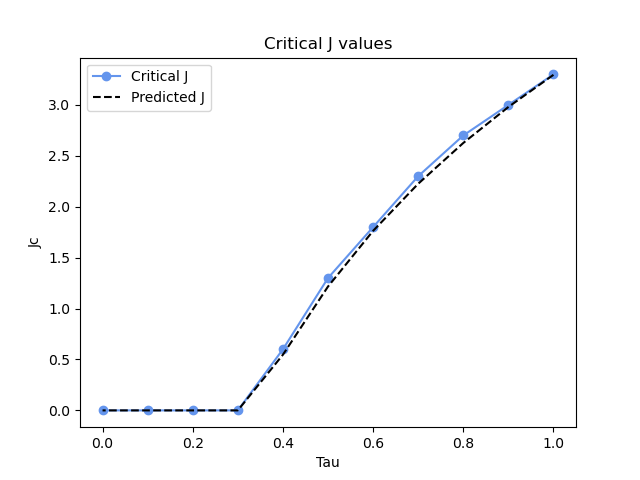
\includegraphics[width=\textwidth]{mf_critical_j}\caption{Mean-field approximation}
        \label{fig:mf_critical_j}
    \end{figure}

\subsection{Simple percolation}\label{subsec:res-simple-percolation}
    In questo caso abbiamo fatto varie simulazioni in base al numero di nodi e al valore di connettività $k$.
    I risultati mostrati in ~\ref{fig:prob_percolation} e ~\ref{fig:prob_percolation_2} mostrano i risultati ottenuti.

    \begin{figure}[h]
        \begin{minipage}{0.5\textwidth}
            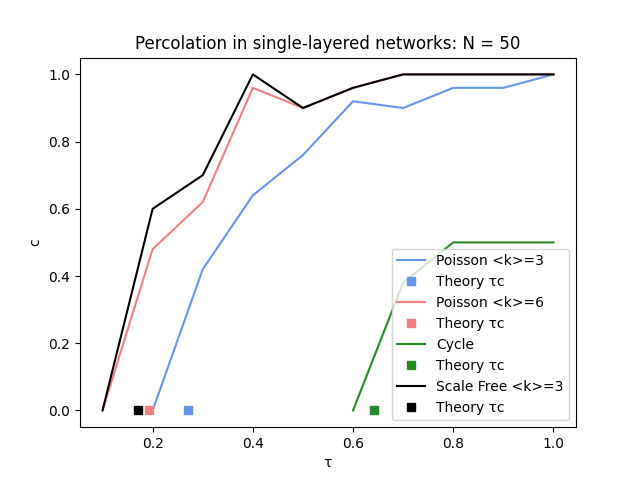
\includegraphics[width=\linewidth]{critical_t}\label{fig:prob_percolation}
        \end{minipage}
        \begin{minipage}{0.5\textwidth}
            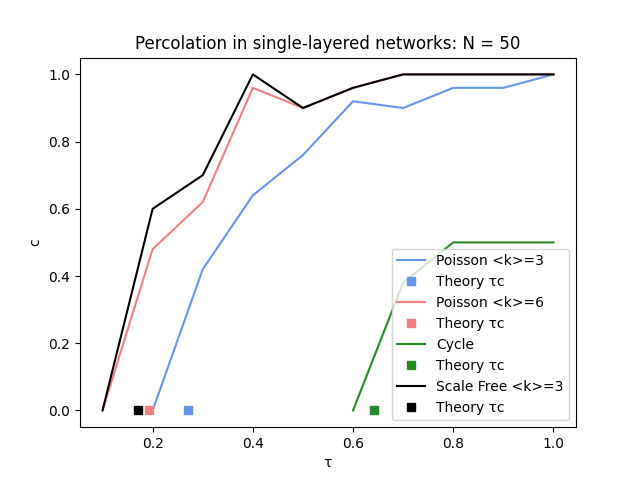
\includegraphics[width=\linewidth]{critical_t}\label{fig:prob_percolation_2}
        \end{minipage}
        \caption{Valutazione della probabilità di percolazione}
    \end{figure}

\subsection{Infezione percezione del rischio}\label{subsec:res-infezione-con-la-percezione-del-rischio}
    Il modello di infezione con la percezione del rischio tiene conto del fatto che le persone possono adottare misure
    precauzioni per proteggersi da una malattia diversamente dal caso precedente.
    Questo metodo è utile per studiare l'effetto della percezione del rischio sulla diffusione di una malattia, ma non
    tiene conto dell'effetto delle informazioni virtuali.

\subsection{Multiplex networks}\label{subsec:res-multiplex-networks}
    I risultati ottenuti dalla simulazione del modello multiplex sono mostrati in figura ~\ref{fig:diagram_phase}.
    Possiamo vedere come all'aumentare di $t$ e $q$ l'infezione si diffonde e non si è in grado di fermarla, infatti i
    valori di $Jc$ aumentano notevolmente.
    Nella visualizzazione del diagramma di fase, possiamo vedere come la curva della soglia di percolazione approssimi 
    un'iperbole.

    \begin{figure}[h]
        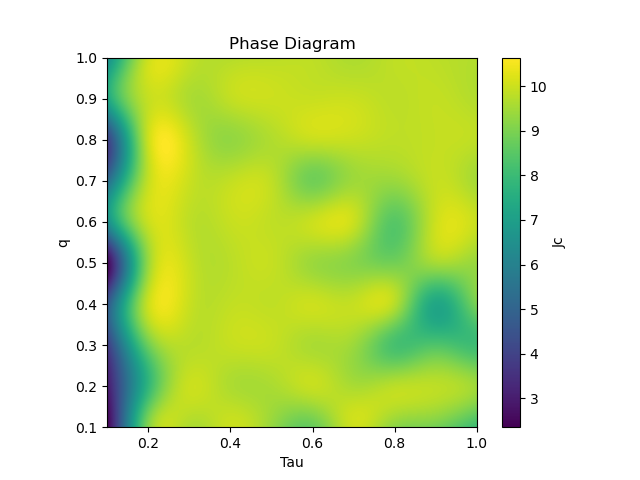
\includegraphics[width=\textwidth]{q_plot}\label{fig:diagram_phase}
        \caption{Diagramma di fase al variare di q e $\tau$}
    \end{figure}
